% Self-contained Beamer supplement to the supplied week42.tex and week43.tex.
% Compile twice with pdflatex. All plotted data are embedded in this file.
% Numerical example: kohn_sham_1d_example.py (NumPy, SciPy, Matplotlib).
\documentclass[aspectratio=169,10pt]{beamer}
\usepackage[utf8]{inputenc}
\usepackage[T1]{fontenc}
\usepackage{lmodern}
\usepackage{amsmath,amssymb,bm,mathtools,booktabs}
\usepackage[most]{tcolorbox}
\usepackage{listings,tikz,pgfplots}
\usetikzlibrary{positioning,arrows.meta}
\pgfplotsset{compat=1.18}
\usetheme{default}
\useinnertheme{rectangles}
\definecolor{uioblue}{RGB}{18,52,86}
\definecolor{teal}{RGB}{0,128,128}
\definecolor{warm}{RGB}{181,73,36}
\definecolor{paleblue}{RGB}{232,240,248}
\definecolor{paleteal}{RGB}{228,244,244}
\definecolor{palewarm}{RGB}{252,238,230}
\setbeamercolor{structure}{fg=uioblue}
\setbeamercolor{title}{fg=uioblue}
\setbeamercolor{frametitle}{fg=uioblue,bg=white}
\setbeamercolor{alerted text}{fg=warm}
\setbeamercolor{block title}{fg=white,bg=uioblue}
\setbeamercolor{block body}{bg=paleblue}
\setbeamercolor{block title example}{fg=white,bg=teal}
\setbeamercolor{block body example}{bg=paleteal}
\setbeamerfont{frametitle}{size=\large,series=\bfseries}
\setbeamerfont{title}{size=\LARGE,series=\bfseries}
\setbeamertemplate{navigation symbols}{}
\setbeamertemplate{frametitle}{%
  \vspace*{0.4em}\insertframetitle\par
  \vspace*{-0.3em}{\color{teal}\rule{\textwidth}{0.6pt}}}
\setbeamertemplate{footline}{%
  \hbox{\begin{beamercolorbox}[wd=\paperwidth,ht=2.4ex,dp=1.2ex,leftskip=1em,rightskip=1em]{structure}%
  \scriptsize FYS4480/9480 -- HK and KS \hfill \insertsectionhead
  \hfill \insertframenumber/\inserttotalframenumber
  \end{beamercolorbox}}}
\setbeamertemplate{itemize items}[circle]
\setbeamertemplate{enumerate items}[default]
\setbeamersize{text margin left=7mm,text margin right=7mm}
\tcbset{left=6pt,right=6pt,top=3pt,bottom=3pt,boxsep=1pt,arc=1pt}
\newcommand{\warnbox}[1]{\begin{tcolorbox}[colback=palewarm,colframe=warm,title={A trap to avoid}]#1\end{tcolorbox}}
\newcommand{\mbbox}[1]{\begin{tcolorbox}[colback=paleblue,colframe=uioblue,title={Many-body connection}]#1\end{tcolorbox}}
\newcommand{\dftbox}[1]{\begin{tcolorbox}[colback=paleteal,colframe=teal,title={Key result}]#1\end{tcolorbox}}
\newcommand{\dd}{\,\mathrm d}
\newcommand{\rr}{\mathbf r}
\newcommand{\ket}[1]{\lvert #1\rangle}
\newcommand{\bra}[1]{\langle #1\rvert}
\newcommand{\avg}[1]{\langle #1\rangle}
\newcommand{\Tr}{\operatorname{Tr}}
\newcommand{\ext}{\mathrm{ext}}
\newcommand{\occ}{\mathrm{occ}}
\newcommand{\xc}{\mathrm{xc}}
\newcommand{\LL}{\mathrm{LL}}
\newcommand{\ens}{\mathrm{ens}}
\newcommand{\inp}{\mathrm{in}}
\newcommand{\out}{\mathrm{out}}
\lstset{language=Python,basicstyle=\ttfamily\footnotesize,
 keywordstyle=\color{uioblue}\bfseries,commentstyle=\color{teal},
 showstringspaces=false,columns=fullflexible,breaklines=true,
 frame=single,rulecolor=\color{paleblue}}
\title{From Hohenberg--Kohn to a working Kohn--Sham calculation}
\subtitle{Detailed proofs, functional derivatives, and a verified SCF example}
\author{FYS4480/FYS9480 -- companion to Weeks 42 and 43}
\institute{Quantum mechanics for many-particle systems\\University of Oslo}
\date{22 October 2026}
\begin{document}

\begin{frame}[plain]
\titlepage
\begin{center}\small
Continuation of the one- and two-body density-matrix derivations.\\
The color scheme and teaching boxes follow the supplied weekly templates.
\end{center}
\end{frame}

\begin{frame}{The route from a theorem to an algorithm}
\begin{enumerate}
\item \textbf{Hohenberg--Kohn I:} why a ground-state density fixes a scalar
external potential, apart from a constant.
\item \textbf{Hohenberg--Kohn II:} why minimizing an exact density functional
recovers the ground-state energy.
\item \textbf{Constrained search:} define the functional on a usable density
domain and handle degenerate states.
\item \textbf{Kohn--Sham:} introduce auxiliary orbitals and derive their equations
with all constraints and functional derivatives shown.
\item \textbf{Implementation:} discretize, build potentials, solve, occupy,
mix, test convergence, and evaluate a consistent energy.
\end{enumerate}
\dftbox{Exact reformulation, approximate functional, finite representation,
and incomplete iteration are four different issues.}
\end{frame}

\section{From RDMs to the density}
\begin{frame}{Where the density-matrix supplement ended}
With $x=(\rr,\sigma)$ and the ordered-pair convention,
\[
 \gamma(x;x')=\avg{\hat\psi^\dagger(x')\hat\psi(x)},\quad
 P(x,y)=\avg{\hat\psi^\dagger(x)\hat\psi^\dagger(y)\hat\psi(y)\hat\psi(x)},
\]
\[
 \Tr\gamma=N,\qquad \int\dd x\dd y\,P=N(N-1),\qquad
 n(\rr)=\sum_\sigma\gamma(\rr\sigma;\rr\sigma).
\]
For a local spin-independent interaction,
\[
 E=T[\gamma]+\int v_{\ext}n\dd^3r
                         +\frac12\int w(\rr,\rr')P(x,y)\dd x\dd y.
\]
\mbbox{For arbitrary states, the local density does not specify the RDMs.
DFT obtains a density functional by minimizing over the missing many-body
information, rather than discarding its energetic consequences.}
\end{frame}

\section{Hohenberg--Kohn I}
\begin{frame}{Specify the family of Hamiltonians before stating the theorem}
Use Hartree atomic units: $\hbar=m_e=e^2/(4\pi\epsilon_0)=1$.
\[
 \hat H[v]=\hat T+\hat W+\hat V[v],\quad
 \hat T=-\frac12\sum_i\nabla_i^2,\quad
 \hat W=\sum_{i<j}\frac1{|\rr_i-\rr_j|},\quad
 \hat V[v]=\sum_i v(\rr_i).
\]
\begin{itemize}
\item Fix $N$, particle statistics, $\hat T$, $\hat W$, the Hilbert space,
and boundary conditions. Change only a scalar local potential $v$.
\item Assume a lower-bounded Hamiltonian with an attained ground-state energy.
Initially assume a nondegenerate ground state.
\item For potential uniqueness, use a continuum potential class with the
needed unique-continuation property; molecular Coulomb potentials are included.
\end{itemize}
\warnbox{The ordinary density-only theorem is not a theorem for arbitrary
nonlocal external operators or magnetic vector potentials. ``Universal''
means independent of $v$ within this fixed problem family.}
\end{frame}

\begin{frame}{The crucial identity: the external energy uses only the density}
For normalized antisymmetric $\Psi$, with $X=(x_2,\ldots,x_N)$,
\[
 n_\Psi(\rr)=N\sum_{\sigma_1}\int\dd X\,
             |\Psi(\rr\sigma_1,X)|^2,\qquad \int n_\Psi\dd^3r=N.
\]
Permutation symmetry of $|\Psi|^2$ makes all $N$ contributions equal:
\begin{align*}
 \avg{\hat V[v]}_\Psi
 &=\sum_i\int\dd x_1\cdots\dd x_N\,
             v(\rr_i)|\Psi(x_1,\ldots,x_N)|^2\\
 &=N\sum_{\sigma_1}\int\dd^3r_1\dd X\,
             v(\rr_1)|\Psi(\rr_1\sigma_1,X)|^2\\
 &=\boxed{\int v(\rr)n_\Psi(\rr)\dd^3r}.
\end{align*}
Only this identity and the variational principle enter the main contradiction.
\end{frame}

\begin{frame}{Rayleigh--Ritz: exactly when is the inequality strict?}
For a normalized trial state, $E_0\leq\avg{\hat H}_\Phi$.
For a discrete spectral expansion $\ket\Phi=\sum_k c_k\ket{\Psi_k}$,
\[
 \avg{\hat H}_\Phi-E_0=\sum_k|c_k|^2(E_k-E_0)\geq0.
\]
\begin{itemize}
\item Equality holds precisely when the trial state lies in the ground-state
eigenspace. The same conclusion holds with continuous spectrum included.
\item With a nondegenerate ground state, equality means
$\Phi=e^{i\theta}\Psi_0$.
\item A different normalized \emph{ray}, not merely a different phase, gives
a strict inequality.
\end{itemize}
\dftbox{To write $E_0<\avg{\hat H}_\Phi$, we must know that $\Phi$ is not
a ground state of this Hamiltonian. Non-degeneracy alone does not establish
that two different potentials have different ground states.}
\end{frame}

\begin{frame}{Why the external potential is determined only up to a constant}
If $v'(\rr)=v(\rr)+C$, then
\[
 \hat H[v']=\hat H[v]+NC,\qquad E_k[v']=E_k[v]+NC.
\]
Every eigenstate and every density is unchanged.
\begin{block}{A gauge choice}
For an isolated atom or molecule one often fixes the zero by specifying the
potential at infinity. Other boundary conditions require their own convention.
\end{block}
\[
 \boxed{n_0\text{ can determine }v\text{ only modulo an additive constant}.}
\]
Changing the constant also shifts Kohn--Sham eigenvalues and the number
multiplier $\mu$. Density and energy differences at the same particle number
remain invariant.
\end{frame}

\begin{frame}{The common-state lemma closes a gap in the short proof}
\small
Suppose the same nonzero $\Psi$ is an eigenstate of $\hat H[v]$ and $\hat H[u]$.
Subtract the two Schr\"odinger equations:
\[
 \left[\sum_i(v-u)(\rr_i)\right]\Psi=(E_v-E_u)\Psi.
\]
For the stated continuum potential class, a relevant nonzero spatial component
of $\Psi$ is nonzero almost everywhere. Hence
\[
 \sum_i\Delta v(\rr_i)=E_v-E_u\quad\text{almost everywhere}.
\]
Fix the other coordinates and vary $\rr_1$:
\[
 \Delta v(\rr_1)=E_v-E_u-\sum_{i=2}^N\Delta v(\rr_i)=C,
 \qquad NC=E_v-E_u.
\]
\warnbox{Nodes on sets of measure zero are allowed. Infinite barriers,
disconnected configuration spaces, lattice models, or arbitrary singular
potentials need separate analysis. This is a stated assumption, not a proof
of unique continuation.}
\end{frame}

\begin{frame}{HK I: assume two inequivalent potentials give the same density}
Let $v$ and $u$ differ by more than a constant. Suppose
\[
 \hat H[v]\Psi_v=E_v\Psi_v,\qquad
 \hat H[u]\Psi_u=E_u\Psi_u,\qquad n_{\Psi_v}=n_{\Psi_u}=n_0.
\]
Both ground states are normalized and nondegenerate.
\begin{enumerate}
\item The common-state lemma implies that their rays are different.
\item Therefore $\Psi_u$ is a strict variational trial state for $\hat H[v]$,
and vice versa.
\item The Hamiltonians differ only by the one-body operator
\[
 \hat H[v]-\hat H[u]=\sum_i[v(\rr_i)-u(\rr_i)].
\]
\end{enumerate}
We can now justify every line of the usual short proof.
\end{frame}

\begin{frame}{HK I: derive the first inequality line by line}
Use $\Psi_u$ as a trial state for the $v$ problem:
\begin{align*}
 E_v
 &<\bra{\Psi_u}\hat H[v]\ket{\Psi_u}
 &&\text{strict Rayleigh--Ritz}\\[1mm]
 &=\bra{\Psi_u}\hat H[u]\ket{\Psi_u}
       +\bra{\Psi_u}\sum_i(v-u)(\rr_i)\ket{\Psi_u}
 &&\text{same }\hat T,\hat W\\[1mm]
 &=E_u+\int[v(\rr)-u(\rr)]n_0(\rr)\dd^3r
 &&\text{same density}.
\end{align*}
\dftbox{The many-body matrix element of the potential difference is exactly
a one-density integral. No determinant factorization or mean-field
approximation has been used.}
\end{frame}

\begin{frame}{HK I: reverse the roles, add, and reach a contradiction}
The two inequalities are
\[
 E_v<E_u+\int(v-u)n_0\dd^3r,
 \qquad E_u<E_v+\int(u-v)n_0\dd^3r.
\]
Adding cancels the density integrals:
\[
 E_v+E_u<E_u+E_v,
\]
which is impossible. Thus
\[
 \boxed{n_0\ \longmapsto\ v\pmod C\ \longmapsto\ \hat H[v]\pmod{NC}.}
\]
With a nondegenerate ground state, the Hamiltonian fixes $\Psi_0$ up to a
phase, and therefore all its expectation values.
\mbbox{This is uniqueness in principle. It neither reconstructs $v$ from
measured $n$ nor supplies an efficient way to solve for $\Psi_0$.}
\end{frame}

\begin{frame}{Degeneracy: replace strictness by an equality argument}
For two ground states with the same density, define
\[
 A=\avg{\hat H[v]}_{\Psi_u}-E_v\geq0,\qquad
 B=\avg{\hat H[u]}_{\Psi_v}-E_u\geq0.
\]
The equal-density identity gives
\[
 A+B=\int(v-u)n_0\dd^3r+\int(u-v)n_0\dd^3r=0.
\]
Hence $A=B=0$: each trial state belongs to both ground-state eigenspaces.
The common-state lemma again implies $v-u=C$.
\begin{itemize}
\item Potential uniqueness survives under the same continuum assumptions.
\item The density need not select one pure state within a degenerate subspace.
\item For ensembles use traces; equality means support only in the ground
eigenspace. Constrained search below handles the variational problem directly.
\end{itemize}
\end{frame}

\section[Density variational principle]{The density variational principle}
\begin{frame}{Which densities may we vary? Three different questions}
\begin{description}
\item[$N$-representable:] some normalized antisymmetric $N$-particle state
with finite kinetic energy produces $n$.
\item[Interacting $v$-representable:] a ground state of $\hat T+\hat W+\hat V[v]$
for an admissible local $v$ produces $n$.
\item[Noninteracting $v$-representable:] a ground state of
$\hat T+\hat V[v_s]$ for a common local $v_s$ produces $n$.
\end{description}
A standard finite-kinetic-energy density domain is
\[
 \mathcal I_N=\{n\geq0:\ \int n=N,\ \sqrt n\in H^1(\mathbb R^3)\}.
\]
$H^1$ requires square integrability of $\sqrt n$ and its weak gradient.
\warnbox{``Every positive function integrating to $N$'' is too broad.
$N$-representability does not imply either form of local-potential ground-state
representability. HK does not prove noninteracting $v$-representability.}
\end{frame}

\begin{frame}{Levy constrained search: define the missing internal energy}
Partition all wave functions according to their density:
\[
 \boxed{F_{\LL}[n]=\inf_{\Psi\to n}\bra\Psi\hat T+\hat W\ket\Psi.}
\]
\begin{itemize}
\item Search over normalized antisymmetric finite-energy states giving the
specified $n$; assign $+\infty$ outside the admissible domain.
\item Many different states may have that density. Select the least internal
energy, rather than claiming they all have the same energy.
\item No external potential appears: $F_{\LL}$ is universal for fixed
statistics, kinetic operator, and interaction.
\item We write an infimum safely; under the standard Coulomb-domain conditions
the constrained minimum is attained.
\end{itemize}
\mbbox{The many-body problem remains inside the constrained search. This
extends the domain of the functional without requiring an explicit inverse
map from a trial density to a potential.}
\end{frame}

\begin{frame}{HK II: regroup Rayleigh--Ritz into a density minimization}
Start with the exact wave-function search:
\begin{align*}
 E_0[v]
 &=\inf_\Psi\left\{\avg{\hat T+\hat W}_\Psi+\int v n_\Psi\dd^3r\right\}\\
 &=\inf_{n\in\mathcal I_N}\inf_{\Psi\to n}
       \left\{\avg{\hat T+\hat W}_\Psi+\int v n\dd^3r\right\}\\
 &=\boxed{\inf_{n\in\mathcal I_N}
       \left\{F_{\LL}[n]+\int v(\rr)n(\rr)\dd^3r\right\}.}
\end{align*}
The external term is constant within each class of states sharing $n$ and
can be taken outside the inner search.
\dftbox{The equality follows by partitioning the same set of trial states.
It does not rely on finding a potential for every trial density.}
\end{frame}

\begin{frame}{HK II: prove the lower bound and prove it is attained}
For every admissible $n$ and every $\Psi\to n$,
\[
 \avg{\hat T+\hat W}_\Psi+\int vn\dd^3r\geq E_0[v].
\]
Take the constrained infimum:
\[
 E_v[n]\equiv F_{\LL}[n]+\int vn\dd^3r\geq E_0[v].
\]
Now insert the actual ground state $\Psi_0\to n_0$:
\[
 F_{\LL}[n_0]\leq\avg{\hat T+\hat W}_{\Psi_0},\qquad E_v[n_0]\leq E_0[v].
\]
Combining the bounds yields
\[
 \boxed{E_v[n_0]=E_0[v]=\min_n E_v[n].}
\]
A unique ground state gives a unique minimizing density. Degenerate ground
states can give several minimizing densities.
\end{frame}

\begin{frame}{Ensembles and the convex functional: keep the definitions distinct}
An $N$-particle ensemble is $\hat{\mathcal D}\geq0$, $\Tr\hat{\mathcal D}=1$.
Define
\[
 F_{\ens}[n]=\inf_{\hat{\mathcal D}\to n}
          \Tr[\hat{\mathcal D}(\hat T+\hat W)].
\]
Mixing ensembles mixes their densities and energies, so
\[
 F_{\ens}[\theta n_1+(1-\theta)n_2]
 \leq\theta F_{\ens}[n_1]+(1-\theta)F_{\ens}[n_2].
\]
In the standard Coulomb framework, Lieb's convex formulation is
\[
 F_L[n]=\sup_v\left\{E_0[v]-\int vn\dd^3r\right\}=F_{\ens}[n]\leq F_{\LL}[n].
\]
They agree at pure-state ground-state densities, but need not agree everywhere.
\dftbox{Below, $F$ denotes the ensemble constrained-search functional.
It gives the same physical ground-state energy and accommodates degenerate
occupations. Do not silently identify a mixed state with one wave function.}
\end{frame}

\begin{frame}{The Euler equation: what the functional derivative means}
Assume the needed derivatives and admissible variations exist. At a minimum,
$\int\delta n\dd^3r=0$ gives
\[
 0=\delta E_v=\int\left[\frac{\delta F}{\delta n(\rr)}+v(\rr)\right]
                           \delta n(\rr)\dd^3r.
\]
For a sufficient class of two-sided admissible variations, the bracket is constant:
\[
 \boxed{\frac{\delta F}{\delta n(\rr)}+v(\rr)=\mu.}
\]
Equivalently vary $E_v[n]-\mu(\int n-N)$. On a fixed-$N$ domain the derivative
is defined only up to a constant, reflected in $\mu$.
\warnbox{Existence of a minimizer does not guarantee differentiability.
The convex statement is $-v\in\partial F[n_0]$, modulo the fixed-$N$
constant: $F[n]\geq F[n_0]-\int v(n-n_0)$. At integer particle numbers,
one-sided chemical potentials may differ.}
\end{frame}

\begin{frame}{What has been established, and what remains unsolved}
\begin{columns}[T]
\column{.48\textwidth}
\begin{block}{Exact statements}
\begin{itemize}
\item A ground-state density determines the scalar potential modulo a constant.
\item Constrained search defines a universal internal-energy functional.
\item Minimizing the exact functional yields the exact energy and a ground-state density.
\end{itemize}
\end{block}
\column{.48\textwidth}
\begin{exampleblock}{Not supplied by these proofs}
\begin{itemize}
\item An explicit or inexpensive formula for $F[n]$.
\item A local noninteracting potential for every admissible density.
\item A practical direct calculation of excitation energies.
\end{itemize}
\end{exampleblock}
\end{columns}
Knowing the Hamiltonian fixes its spectrum in principle. The ground-state
variational procedure does not itself compute that spectrum; auxiliary KS
eigenvalues need separate interpretation.
\end{frame}

\begin{frame}{Pause to think: locate the assumptions}
\begin{tcolorbox}[colback=palewarm,colframe=warm,title={Discuss with a neighbor}]
\begin{enumerate}
\item Why does the contradiction not distinguish $v$ from $v+C$?
\item Does a degenerate ground-state density specify a unique wave function?
\item Why is minimizing over all normalized positive functions not a complete
statement of the density variational principle?
\item Does constrained search provide an explicit formula for $F[n]$?
\end{enumerate}
\end{tcolorbox}
\end{frame}

\begin{frame}{Answer: uniqueness, domain, and computation are different issues}
\begin{enumerate}
\item The states are unchanged by $NC$; in the contradiction the trial state
then need not give a strict inequality.
\item No. Potential uniqueness can fix the Hamiltonian and its ground-state
space without selecting a particular state in that space.
\item Trial densities must come from admissible finite-energy states; otherwise
the constrained-search energy is not finite.
\item No. It defines the exact quantity and proves its variational role.
Evaluating the constrained search is still a many-body calculation.
\end{enumerate}
\dftbox{Kohn--Sham addresses the computational representation. Approximating
the exchange-correlation functional is a later, separate step.}
\end{frame}

\section{Kohn--Sham derivation}
\begin{frame}{Why put orbitals back into a density theory?}
The local Thomas--Fermi kinetic approximation in 3D is
\[
 T_{\rm TF}[n]=\frac3{10}(3\pi^2)^{2/3}\int n^{5/3}\dd^3r
\]
for an unpolarized electron gas. It has no explicit orbital shell structure.
Kohn and Sham instead compute an auxiliary kinetic energy from orbitals:
\[
 T_s=\sum_i f_i\bra{\phi_i}-\frac12\nabla^2\ket{\phi_i},\qquad
 n(\rr)=\sum_i f_i\sum_\sigma|\phi_i(\rr\sigma)|^2.
\]
\begin{itemize}
\item $T_s$ is exact for the auxiliary noninteracting problem, not generally
equal to the interacting kinetic energy $T$.
\item Orbitals represent $T_s$ implicitly as a functional of $n$.
\item They recover noninteracting shell structure while retaining the density
as the target quantity.
\end{itemize}
\end{frame}

\begin{frame}{Define the noninteracting kinetic functional carefully}
Using orthonormal spin orbitals and ensemble occupations,
\[
 \boxed{T_s[n]=\inf_{\{f_i,\phi_i\}\to n}
       \sum_i f_i\bra{\phi_i}\hat t\ket{\phi_i},}
 \qquad 0\leq f_i\leq1,\quad \sum_i f_i=N.
\]
Restricting this search to integer occupations gives the determinant
constrained search with density $n$.
\begin{block}{Representation versus ground-state representation}
Writing a density using orbitals is weaker than finding a common local
potential whose noninteracting ground state has that density.
The differential KS construction assumes a suitable supporting potential
and derivatives, or their ensemble/subgradient counterparts.
\end{block}
We first derive the orbital equations for unit occupations of the occupied
spin orbitals. Degenerate and spin-resolved occupations are added afterward.
\end{frame}

\begin{frame}{Define exchange-correlation so the energy decomposition is exact}
For a fixed symmetric interaction $w$, set
\[
 E_H[n]=\frac12\iint n(\rr)w(\rr,\rr')n(\rr')\dd^3r\dd^3r',
 \qquad \boxed{E_{\xc}[n]=F[n]-T_s[n]-E_H[n].}
\]
Therefore
\[
 \boxed{E_v[n]=T_s[n]+\int v_{\ext}n\dd^3r+E_H[n]+E_{\xc}[n].}
\]
At a constrained-search minimizing interacting state,
\[
 E_{\xc}=(T-T_s)+(W-E_H).
\]
\begin{itemize}
\item Correlation includes a kinetic contribution. It is not just the pair-density cumulant.
\item No approximation has yet been made, and no general theorem says this remainder is small.
\item In practice replace $E_{\xc}$ by a chosen approximation and solve the resulting problem consistently.
\end{itemize}
\end{frame}

\begin{frame}{Derive the Hartree potential: vary both density factors}
For symmetric $w(\rr,\rr')$,
\begin{align*}
 \delta E_H
 &=\frac12\iint w(\rr,\rr')
 [\delta n(\rr)n(\rr')+n(\rr)\delta n(\rr')]\dd^3r\dd^3r'\\
 &=\int\left[\int w(\rr,\rr')n(\rr')\dd^3r'\right]
                          \delta n(\rr)\dd^3r.
\end{align*}
Thus
\[
 \boxed{v_H(\rr)=\frac{\delta E_H}{\delta n(\rr)}
       =\int w(\rr,\rr')n(\rr')\dd^3r',}\qquad \int n v_H=2E_H.
\]
For 3D Coulomb electrons, $w=1/|\rr-\rr'|$. For the softened 1D model later,
use its own interaction kernel; the formal variation is unchanged.
\end{frame}

\begin{frame}{The variational object includes all orthonormality constraints}
For occupied unit-occupation spin orbitals,
\[
 n(\rr)=\sum_{i\in\occ}\sum_\sigma|\phi_i(\rr\sigma)|^2,
 \qquad \avg{\phi_i|\phi_j}=\delta_{ij}.
\]
Write the orbital energy and constrained Lagrangian:
\begin{align*}
 \mathcal E[\{\phi_i\}]&=\sum_{i\in\occ}\bra{\phi_i}\hat t\ket{\phi_i}
       +E_{\ext}[n]+E_H[n]+E_{\xc}[n],\\
 \mathcal L&=\mathcal E-\sum_{ij}\Lambda_{ij}
          (\avg{\phi_j|\phi_i}-\delta_{ji}),\qquad \Lambda=\Lambda^\dagger.
\end{align*}
\mbbox{Use a matrix of multipliers, not independent scalar orbital energies
at the outset. Off-diagonal constraints enforce mutual orthogonality,
just as in the Hartree--Fock variation.}
Treat $\phi_i$ and $\phi_i^*$ as independent variables during variation.
\end{frame}

\begin{frame}{Carry out each orbital derivative}
For the variation with respect to $\phi_i^*(x)$,
\[
 \frac{\delta n(\rr)}{\delta\phi_i^*(x)}
 =\delta^{(3)}(\rr-\mathbf r_x)\phi_i(x),\qquad x=(\mathbf r_x,\sigma_x).
\]
The contributions are
\begin{align*}
 \frac{\delta T_s}{\delta\phi_i^*(x)}&=\hat t\phi_i(x),\\
 \frac{\delta E_{\ext}}{\delta\phi_i^*(x)}&=v_{\ext}(\rr)\phi_i(x),\\
 \frac{\delta(E_H+E_{\xc})}{\delta\phi_i^*(x)}
       &=[v_H(\rr)+v_{\xc}(\rr)]\phi_i(x),
 \qquad v_{\xc}=\frac{\delta E_{\xc}}{\delta n},\\
 \frac{\delta}{\delta\phi_i^*(x)}\sum_{jk}\Lambda_{jk}\avg{\phi_k|\phi_j}
       &=\sum_j\Lambda_{ji}\phi_j(x).
\end{align*}
Here a density-functional derivative and the chain rule turn the interaction
functional into an orbital equation.
\end{frame}

\begin{frame}{Stationarity and the canonical Kohn--Sham equations}
Setting the derivative of $\mathcal L$ to zero gives
\[
 \hat h_s\phi_i=\sum_j\Lambda_{ji}\phi_j,\qquad
 \hat h_s=-\frac12\nabla^2+v_s(\rr),
\]
\[
 v_s=v_{\ext}+v_H[n]+v_{\xc}[n].
\]
The density and energy are invariant under unitary rotations among equally
occupied orbitals. Diagonalize the Hermitian $\Lambda$ in that subspace:
\[
 \boxed{\left[-\frac12\nabla^2+v_{\ext}+v_H[n]+v_{\xc}[n]\right]\phi_i
          =\epsilon_i\phi_i,\qquad n=\sum_{i\in\occ,\sigma}|\phi_i|^2.}
\]
\dftbox{The problem is nonlinear: the density defines the potential, the
potential defines the orbitals, and the occupied orbitals define the density.}
\end{frame}

\begin{frame}{Check the construction against the density Euler equation}
For the auxiliary noninteracting ground state,
\[
 \frac{\delta T_s}{\delta n}+v_s=\mu_s.
\]
For the interacting density minimization,
\[
 \frac{\delta F}{\delta n}+v_{\ext}=\mu.
\]
Since $F=T_s+E_H+E_{\xc}$, subtraction gives
\[
 v_s(\rr)=v_{\ext}(\rr)+v_H(\rr)+v_{\xc}(\rr)+\mu_s-\mu.
\]
The final constant is absorbed into the potential gauge.
\begin{block}{Two ways to see the same construction}
The constrained orbital variation yields the differential equations.
The density Euler equations explain why the effective potential has exactly
these three contributions, when the required derivatives exist.
\end{block}
\end{frame}

\begin{frame}{Occupations and spin: avoid hidden factors of two}
For spin orbitals, $0\leq f_i\leq1$ and $\sum_i f_i=N$.
At zero temperature, occupation minimization fills the lowest levels:
\[
 f_i=1\ (\epsilon_i<\mu),\quad f_i=0\ (\epsilon_i>\mu),\quad
 0\leq f_i\leq1\ (\epsilon_i=\mu).
\]
For collinear spin DFT,
\[
 n_\sigma(\rr)=\sum_i f_{i\sigma}|\phi_{i\sigma}(\rr)|^2,\quad
 v_{\xc,\sigma}=\frac{\delta E_{\xc}[n_\uparrow,n_\downarrow]}{\delta n_\sigma},
 \quad n=n_\uparrow+n_\downarrow.
\]
\begin{itemize}
\item Doubly occupied \emph{spatial} orbitals use occupations up to 2 instead.
Do not also sum spin a second time.
\item The numerical model later is \emph{spinless}: one particle per orbital.
\item Finite-temperature Fermi occupations minimize a free energy containing
an entropy term. Smearing is not an undocumented zero-temperature identity.
\end{itemize}
\end{frame}

\begin{frame}{Derive the total energy: why the eigenvalue sum is wrong}
Multiply each KS equation by $f_i\phi_i^*$, integrate, and sum:
\[
 \sum_i f_i\epsilon_i=T_s+\int n v_{\ext}+\int n v_H+\int n v_{\xc}
                     =T_s+E_{\ext}+2E_H+\int n v_{\xc}.
\]
Subtract the actual energy $E=T_s+E_{\ext}+E_H+E_{\xc}$:
\[
 \boxed{E=\sum_i f_i\epsilon_i-E_H[n]+E_{\xc}[n]
                                  -\int n(\rr)v_{\xc}(\rr)\dd^3r.}
\]
For spin DFT replace the last integral by $\sum_\sigma\int n_\sigma v_{\xc,\sigma}$.
\begin{itemize}
\item The Hartree potential counts each pair twice in the eigenvalue sum.
\item $v_{\xc}$ is a derivative; its expectation is not $E_{\xc}$.
\item Add $E_{NN}$ for clamped-nuclei molecular/crystal total energies.
\end{itemize}
This is a consistency identity for the same orbitals, potential, and density.
\end{frame}

\begin{frame}{Local operator does not mean a local density functional}
In conventional KS, $v_{\xc}([n];\rr)$ multiplies an orbital at $\rr$:
\[
 (\hat v_{\xc}\phi)(\rr)=v_{\xc}([n];\rr)\phi(\rr).
\]
Its value may nevertheless depend on the density everywhere.
\begin{center}\small
\begin{tabular}{@{}lll@{}}
\toprule
Object & Dependence & Action on an orbital\\\midrule
$v_H[n](\rr)$ & integral over $n(\rr')$ & multiplicative\\
$v_{\xc}^{\rm LDA}$ & value of $n$ at $\rr$ & multiplicative\\
$v_{\xc}^{\rm GGA}$ & $n$ and spatial derivatives & multiplicative\\
Exact local KS $v_{\xc}$ & generally nonlocal in $n$ & multiplicative\\
HF Fock exchange & off-diagonal one-body RDM & integral operator\\\bottomrule
\end{tabular}
\end{center}
\warnbox{Exact KS is not inherently approximate. LDA/GGA are approximation
choices for its unknown functional. Nonlocal density dependence and a
nonlocal orbital operator are different meanings of ``nonlocal''.}
\end{frame}

\section[Functionals]{Choosing and differentiating a functional}
\begin{frame}{LDA: differentiate the energy per volume, not per particle}
Let $\epsilon_{\xc}(n)$ be the uniform-gas energy \emph{per particle}.
The LDA approximation is
\[
 E_{\xc}^{\rm LDA}[n]=\int f_{\xc}(n(\rr))\dd^3r,
 \qquad f_{\xc}(n)=n\epsilon_{\xc}(n).
\]
Varying at each point gives
\begin{align*}
 \delta E_{\xc}&=\int[\epsilon_{\xc}(n)+n\epsilon_{\xc}'(n)]\delta n\dd^3r,\\
 \boxed{v_{\xc}^{\rm LDA}(\rr)}
   &\boxed{=\frac{\dd[n\epsilon_{\xc}(n)]}{\dd n}
          =\epsilon_{\xc}(n)+n\epsilon_{\xc}'(n).}
\end{align*}
If correlation is parameterized by $r_s\propto n^{-1/3}$ in 3D,
\[
 v_c=\epsilon_c(r_s)-\frac{r_s}{3}\frac{\dd\epsilon_c}{\dd r_s}.
\]
Energy and potential must be derived from the \emph{same} functional or interpolant.
\end{frame}

\begin{frame}{Derive the 3D exchange potential and check the units}
For a spin-unpolarized 3D gas,
\[
 k_F=(3\pi^2n)^{1/3},\qquad
 \epsilon_x=-\frac{3k_F}{4\pi}
            =-\frac34\left(\frac3\pi\right)^{1/3}n^{1/3}.
\]
Therefore
\[
 E_x^{\rm LDA}=-C_x\int n^{4/3}\dd^3r,\quad
 C_x=\frac34\left(\frac3\pi\right)^{1/3},\quad
 \boxed{v_x=-\left(\frac3\pi\right)^{1/3}n^{1/3}=\frac43\epsilon_x.}
\]
With $n=3/(4\pi r_s^3)$,
\[
 \epsilon_x=-\frac{0.4581653}{r_s}\ {\rm Ha}
           =-\frac{0.9163306}{r_s}\ {\rm Ry}.
\]
\warnbox{This is the 3D, two-spin-species formula. The 1D spinless model
requires a different uniform reference and functional, not a reused $n^{1/3}$ law.}
\end{frame}

\begin{frame}{GGA: show the integration by parts explicitly}
For $E_{\xc}^{\rm GGA}=\int f(n,\nabla n)\dd^3r$,
\begin{align*}
 \delta E_{\xc}
 &=\int\left[\frac{\partial f}{\partial n}\delta n
       +\frac{\partial f}{\partial(\nabla n)}\cdot\nabla\delta n\right]\dd^3r\\
 &=\int\left[\frac{\partial f}{\partial n}
       -\nabla\cdot\frac{\partial f}{\partial(\nabla n)}\right]\delta n\dd^3r
       +\text{surface term}.
\end{align*}
For appropriate decaying or periodic boundary conditions,
\[
 \boxed{v_{\xc}^{\rm GGA}=\frac{\partial f}{\partial n}
                       -\nabla\cdot\frac{\partial f}{\partial(\nabla n)}.}
\]
For $q=|\nabla n|^2$ and $f=f(n,q)$, this becomes
$v_{\xc}=f_n-2\nabla\cdot(f_q\nabla n)$.
\mbbox{The boundary condition and discrete derivative must match the energy
discretization. A continuum derivative copied into an inconsistent numerical
scheme can destroy variational consistency.}
\end{frame}

\begin{frame}{Hartree--Fock, exact-exchange KS, and generalized KS}
\begin{itemize}
\item \textbf{HF:} minimize the expectation of the true Hamiltonian over
determinants. The exchange variation gives a nonlocal Fock operator.
\item \textbf{Conventional KS:} reproduce the density using a multiplicative
potential. Exact $E_{\xc}$ would be exact within the representation assumptions.
\item \textbf{Exact exchange via OEP:} an orbital exchange functional can be
used with a local optimized effective potential; it need not yield HF orbitals.
\item \textbf{Hybrids/generalized KS:} direct orbital variation of an exchange
mixture usually produces a nonlocal operator. Do not apply local-KS energy
or spectral formulas unchanged.
\end{itemize}
\warnbox{There is no general theorem that the same fixed percentage of exchange
is recovered, that local-exchange energy always lies above HF, or that any
hybrid completely removes self-interaction. Such comparisons depend on the
functional, system, and representation.}
\end{frame}

\section{The practical SCF algorithm}
\begin{frame}{The nonlinear problem is a fixed point}
Define the output-density map $\mathcal F[n]$ by building and solving
the KS Hamiltonian at an input density. The target satisfies
\[
 \boxed{n_* = \mathcal F[n_*].}
\]
\begin{center}
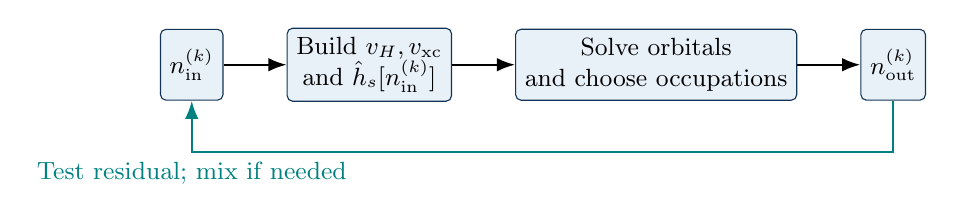
\begin{tikzpicture}[node distance=7mm and 8mm,
 box/.style={draw=uioblue,fill=paleblue,rounded corners=2pt,
 minimum height=9mm,align=center,font=\small}, >=Latex]
\node[box] (n) {$n_{\inp}^{(k)}$};
\node[box,right=of n] (v) {Build $v_H,v_{\xc}$\\and $\hat h_s[n_{\inp}^{(k)}]$};
\node[box,right=of v] (solve) {Solve orbitals\\and choose occupations};
\node[box,right=of solve] (out) {$n_{\out}^{(k)}$};
\draw[->,thick] (n)--(v);\draw[->,thick] (v)--(solve);\draw[->,thick] (solve)--(out);
\draw[->,thick,teal] (out.south)--++(0,-.65)-|node[below,pos=.5,font=\small]
 {Test residual; mix if needed} (n.south);
\end{tikzpicture}
\end{center}
\vspace{3mm}
At fixed occupations, the solve is linear; the repeated density--potential
update is the nonlinear part. A small eigenproblem residual alone is not
self-consistency.
\end{frame}

\begin{frame}{Basis implementation: the generalized eigenvalue problem}
Expand $\phi_i(x)=\sum_\mu C_{\mu i}\chi_\mu(x)$. Define
\[
 S_{\mu\nu}=\int\chi_\mu^*\chi_\nu\dd x,\quad
 H_{\mu\nu}[n]=\int\chi_\mu^*(\hat t+v_{\ext}+v_H+v_{\xc})\chi_\nu\dd x.
\]
The projected equations and normalization are
\[
 \boxed{H C=S C\varepsilon,\qquad C^\dagger S C=I.}
\]
With $D_{\mu\nu}=\sum_i f_i C_{\mu i}C_{\nu i}^*$,
\[
 n(\rr)=\sum_{\mu\nu,\sigma}\chi_\mu(\rr\sigma)D_{\mu\nu}
                            \chi_\nu^*(\rr\sigma),\qquad \Tr(DS)=N.
\]
For $S>0$, orthogonalize with $X=S^{-1/2}$ and solve $X^\dagger H X$.
Remove or control nearly dependent basis directions before taking $S^{-1/2}$.
\end{frame}

\begin{frame}{Grid implementation: quadrature weights belong in the density}
For a uniform 1D grid $x_j$ with spacing $h$ and Dirichlet boundaries,
\[
 -\frac12\phi''(x_j)\simeq
 \frac{2\phi_j-\phi_{j-1}-\phi_{j+1}}{2h^2}.
\]
If the matrix eigensolver normalizes $\sum_j|u_{ji}|^2=1$, then
\[
 \phi_i(x_j)=u_{ji}/\sqrt h,\qquad
 n_j=\frac1h\sum_i f_i|u_{ji}|^2,\qquad h\sum_j n_j=N.
\]
For general quadrature weights $w_j$, use the corresponding weighted overlap
or transformed coefficients consistently.
\warnbox{Do not normalize orbitals with one quadrature and integrate density
or energy with another without checking consistency. Refine the grid and
enlarge the box independently; a converged SCF loop cannot repair either error.}
\end{frame}

\begin{frame}{Build the Hartree field with the correct kernel and boundaries}
In a quadrature representation,
\[
 (v_H)_j=\sum_k w_k\,w(x_j,x_k)n_k,\qquad
 E_H=\frac12\sum_j w_j n_j(v_H)_j.
\]
For Coulomb electrons in \emph{three dimensions}, an equivalent formulation is
\[
 \nabla^2v_H(\rr)=-4\pi n(\rr),\qquad
 v_H(\rr)\sim N/|\rr|\quad\text{for an isolated localized density}.
\]
\begin{itemize}
\item Isolated systems need isolated/open-boundary electrostatics.
\item Periodic cells require a consistent neutrality and zero-mode convention.
Include the ion/background terms in a physical periodic total energy.
\item The softened 1D kernel $1/\sqrt{(x-x')^2+a^2}$ is a convolution;
it is not the solution of this 3D Poisson equation on a line.
\end{itemize}
\end{frame}

\begin{frame}{Density mixing: stability follows from a linearized map}
Let the unmixed residual be $R^{(k)}=n_{\out}^{(k)}-n_{\inp}^{(k)}$.
Linear mixing uses
\[
 n_{\inp}^{(k+1)}=n_{\inp}^{(k)}+\alpha R^{(k)}
                  =(1-\alpha)n_{\inp}^{(k)}+\alpha n_{\out}^{(k)}.
\]
Near a fixed point, with $J=\delta\mathcal F/\delta n$,
\[
 \delta n^{(k+1)}\simeq[(1-\alpha)I+\alpha J]\delta n^{(k)}.
\]
Local linear convergence is guaranteed when the spectral radius is less than
one on allowed variations.
\begin{itemize}
\item $0<\alpha\leq1$ preserves positivity and particle number if both inputs have them.
\item Small $\alpha$ can damp oscillations; it is not a universal convergence guarantee.
\item Pulay/DIIS and preconditioned mixing accelerate difficult cases but need safeguards.
\item Test $R$, not just the mixed step $\alpha R$, which can be made small artificially.
\end{itemize}
\end{frame}

\begin{frame}[fragile]{A practical algorithm, with consistent bookkeeping}
\begin{lstlisting}
n_in = initial_density(N)       # nonnegative; integral = N
E_previous = None
for k in range(max_iterations):
    vH, vxc = potentials(n_in)
    eps, orbitals = solve_KS(vext + vH + vxc)
    f = occupations(eps, N)     # use the stated spin convention
    n_out = density(orbitals, f)
    R = n_out - n_in
    E = direct_energy(orbitals, f, n_out)
    if residual_small(R) and energy_stable(E, E_previous):
        break
    n_in = (1-alpha)*n_in + alpha*n_out
    E_previous = E
else:
    raise ConvergenceError
\end{lstlisting}
\small Rebuild final potentials and check orbital/energy consistency.
A maximum-iteration exit is a failure report, not convergence.
\end{frame}

\begin{frame}{During SCF, compute an energy from one consistent output state}
Orbitals obtained from $\hat h_s[n_{\inp}]$ give $n_{\out}$.
Evaluate the direct functional as
\[
 E^{(k)}=\sum_i f_i\bra{\phi_i^{(k)}}\hat t+v_{\ext}\ket{\phi_i^{(k)}}
                   +E_H[n_{\out}^{(k)}]+E_{\xc}[n_{\out}^{(k)}].
\]
This is the chosen functional evaluated on the actual output orbitals/density.
Away from self-consistency,
\[
 \sum_i f_i\epsilon_i^{(k)}=T_s^{(k)}+E_{\ext}[n_{\out}]
                  +\int n_{\out}(v_H[n_{\inp}]+v_{\xc}[n_{\inp}]).
\]
\warnbox{The usual double-counting formula cannot combine old eigenvalues
with newly mixed density corrections arbitrarily. At convergence, the
direct and eigenvalue-corrected energies must agree within an energy-consistency
tolerance compatible with the density and orbital residuals.}
\end{frame}

\begin{frame}{Convergence checks: three numerical questions, then physics}
\begin{center}\small
\begin{tabular}{@{}lll@{}}
\toprule
Check & Example diagnostic & What it tests\\\midrule
Particle number & $|\int n-N|$ & occupations and quadrature\\
Orthonormality & $\|C^\dagger S C-I\|$ & basis/eigensolver normalization\\
SCF consistency & $\|n_{\out}-n_{\inp}\|$ & nonlinear fixed point\\
Orbital stationarity & $\|HC-SC\varepsilon\|$ & final KS equations\\
Energy bookkeeping & $|E_{\rm direct}-E_{\rm eig}|$ & consistent functional terms\\
Representation & box/grid/basis refinement & discretization error\\\bottomrule
\end{tabular}
\end{center}
Also try different starting densities and relevant spin/symmetry sectors.
\dftbox{A self-consistent solution may be a local stationary solution, not
the global functional minimum. Tiny numerical residuals do not establish
the accuracy of the approximate exchange-correlation functional.}
\end{frame}

\section{Verified one-dimensional example}
\begin{frame}{Use the Week-43 Hamiltonian, with its own exchange functional}
Take $N$ spinless fermions in oscillator units:
\[
 \hat h_0=-\frac12\frac{\dd^2}{\dd x^2}+\frac{x^2}{2},\qquad
 w(s)=\frac1{\sqrt{s^2+a^2}},\qquad a=0.5.
\]
Use the first $M$ harmonic-oscillator functions as a Galerkin basis.
The numerical functional is
\[
 E=\sum_{i=1}^{N}\bra{\phi_i}\hat h_0\ket{\phi_i}
        +\frac12\iint n(x)w(x-y)n(y)\dd x\dd y+\int e_x(n(x))\dd x.
\]
\begin{itemize}
\item Exchange-only LDA: no correlation functional is included.
\item The uniform reference is 1D and spinless; each orbital holds one particle.
\item Calculations below were recomputed for this supplement, using a refined
uniform-exchange evaluation. Do not mix their last digits with older tables.
\end{itemize}
\end{frame}

\begin{frame}{Derive the 1D uniform-gas exchange energy}
The filled interval $-k_F\leq k\leq k_F$ gives
\[
 n=\int_{-k_F}^{k_F}\frac{\dd k}{2\pi}=\frac{k_F}{\pi},\qquad
 \gamma(s)=\int_{-k_F}^{k_F}\frac{\dd k}{2\pi}e^{iks}
                         =\frac{\sin(k_Fs)}{\pi s}.
\]
For a determinant, $P=n^2-|\gamma(s)|^2$. Its exchange energy per length is
\begin{align*}
 e_x(n)&=-\frac12\int_{-\infty}^{\infty}w(s)|\gamma(s)|^2\dd s\\
       &=-\int_0^\infty\frac1{\sqrt{s^2+a^2}}
                         \left[\frac{\sin(\pi ns)}{\pi s}\right]^2\dd s.
\end{align*}
\[
 \boxed{\epsilon_x(n)=e_x(n)/n,\qquad E_x^{\rm LDA}=\int e_x(n(x))\dd x,
        \qquad v_x(n)=e_x'(n).}
\]
The uniform Hartree energy needs a neutralizing background; the exchange
integral is finite. The finite trapped Hartree term is evaluated directly.
\end{frame}

\begin{frame}{Tabulate energy and derive the potential consistently}
For $w(s)=1/\sqrt{s^2+a^2}$, its Fourier transform is
$\widetilde w(q)=2K_0(a|q|)$. With $Q=2\pi n$,
\[
 e_x(n)=-\frac1{2\pi^2}\int_0^Q(Q-q)K_0(aq)\dd q,
 \qquad v_x(n)=-\frac1\pi\int_0^QK_0(aq)\dd q.
\]
$K_0$ is the modified Bessel function; its logarithmic endpoint singularity
is integrable. The companion code tabulates $e_x$ and its slope, then uses
the derivative of the \emph{same} Hermite interpolant in SCF.
\begin{center}\small
\begin{tabular}{@{}rrr@{}}\toprule
$n$ & $\epsilon_x(n)$ & $v_x(n)$\\\midrule
0.05 & $-0.1735293$ & $-0.2973727$\\
0.20 & $-0.4233271$ & $-0.6578909$\\
0.80 & $-0.7588439$ & $-0.9658763$\\
2.50 & $-0.9189555$ & $-0.9998969$\\\bottomrule
\end{tabular}
\end{center}
Both tend to $-1/(2a)=-1$ at high density; neither follows the 3D power law.
\end{frame}

\begin{frame}{Assemble the finite-basis matrices using one quadrature}
On quadrature nodes $x_j$ with weights $w_j$, let $B_{j\mu}=\chi_\mu(x_j)$.
Use $S=B^\dagger W B$ and orthogonalize if needed. In the orthogonalized basis,
\[
 F[n]=h_0+B^\dagger W\operatorname{diag}(v_H[n]+v_x[n])B,
 \quad FC=C\varepsilon,\quad C^\dagger C=I.
\]
For spinless integer occupations,
\[
 n_j=\sum_{i=1}^{N}|(BC)_{ji}|^2,\quad
 (v_H)_j=\sum_k w_k\frac{n_k}{\sqrt{(x_j-x_k)^2+a^2}}.
\]
The direct energy is
\[
 E=\Tr(Dh_0)+\frac12\sum_j w_j n_j(v_H)_j+\sum_jw_j e_x(n_j),
 \qquad D=C_{\occ}C_{\occ}^\dagger.
\]
Baseline settings: $M=8$, $x\in[-8,8]$, 401 Simpson nodes,
601 exchange-table nodes up to $n=3$, mixing $\alpha=0.30$.
\end{frame}

\begin{frame}{The computed densities retain orbital shell structure}
\begin{columns}[T]
\column{.65\textwidth}
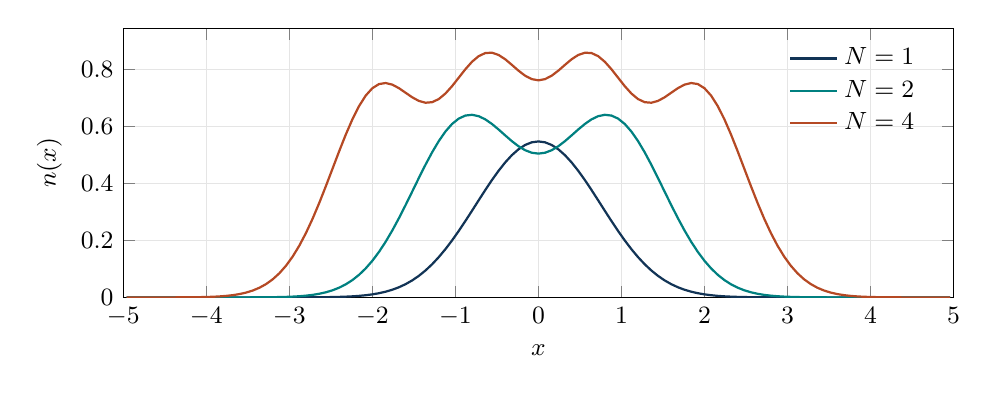
\begin{tikzpicture}
\begin{axis}[width=\linewidth,height=5.0cm,xlabel={$x$},ylabel={$n(x)$},xmin=-5,xmax=5,ymin=0,grid=major,grid style={gray!20},legend style={font=\small,draw=none,fill=none},legend pos=north east,tick label style={font=\small},label style={font=\small}]
\addplot[thick,uioblue] coordinates {(-4.960,1.6115204e-09) (-4.880,2.849149e-09) (-4.800,4.9589871e-09) (-4.720,8.4983549e-09) (-4.640,1.4342669e-08) (-4.560,2.3844916e-08) (-4.480,3.9064625e-08) (-4.400,6.3093525e-08) (-4.320,1.0051643e-07) (-4.240,1.5806359e-07) (-4.160,2.4553932e-07) (-4.080,3.7715771e-07) (-4.000,5.7349155e-07) (-3.920,8.6436064e-07) (-3.840,1.2931781e-06) (-3.760,1.9235764e-06) (-3.680,2.8496062e-06) (-3.600,4.2115359e-06) (-3.520,6.2203947e-06) (-3.440,9.1960984e-06) (-3.360,1.3626506e-05) (-3.280,2.0258403e-05) (-3.200,3.0236561e-05) (-3.120,4.5314001e-05) (-3.040,6.8165701e-05) (-2.960,0.00010284909) (-2.880,0.00015546727) (-2.800,0.00023510348) (-2.720,0.00035510564) (-2.640,0.00053480356) (-2.560,0.00080173422) (-2.480,0.001194426) (-2.400,0.0017657452) (-2.320,0.0025867324) (-2.240,0.003750754) (-2.160,0.0053776617) (-2.080,0.0076175117) (-2.000,0.010653253) (-1.920,0.014701682) (-1.840,0.020011903) (-1.760,0.026860579) (-1.680,0.035543373) (-1.600,0.046362275) (-1.520,0.059608874) (-1.440,0.075544094) (-1.360,0.094375418) (-1.280,0.11623311) (-1.200,0.14114727) (-1.120,0.16902787) (-1.040,0.19964974) (-0.960,0.23264437) (-0.880,0.2674999) (-0.800,0.30356996) (-0.720,0.34009143) (-0.640,0.37621021) (-0.560,0.4110138) (-0.480,0.44356857) (-0.400,0.47295959) (-0.320,0.49833065) (-0.240,0.5189222) (-0.160,0.53410522) (-0.080,0.54340926) (0.000,0.54654342) (0.080,0.54340926) (0.160,0.53410522) (0.240,0.5189222) (0.320,0.49833065) (0.400,0.47295959) (0.480,0.44356857) (0.560,0.4110138) (0.640,0.37621021) (0.720,0.34009143) (0.800,0.30356996) (0.880,0.2674999) (0.960,0.23264437) (1.040,0.19964974) (1.120,0.16902787) (1.200,0.14114727) (1.280,0.11623311) (1.360,0.094375418) (1.440,0.075544094) (1.520,0.059608874) (1.600,0.046362275) (1.680,0.035543373) (1.760,0.026860579) (1.840,0.020011903) (1.920,0.014701682) (2.000,0.010653253) (2.080,0.0076175117) (2.160,0.0053776617) (2.240,0.003750754) (2.320,0.0025867324) (2.400,0.0017657452) (2.480,0.001194426) (2.560,0.00080173422) (2.640,0.00053480356) (2.720,0.00035510564) (2.800,0.00023510348) (2.880,0.00015546727) (2.960,0.00010284909) (3.040,6.8165701e-05) (3.120,4.5314001e-05) (3.200,3.0236561e-05) (3.280,2.0258403e-05) (3.360,1.3626506e-05) (3.440,9.1960984e-06) (3.520,6.2203947e-06) (3.600,4.2115359e-06) (3.680,2.8496062e-06) (3.760,1.9235764e-06) (3.840,1.2931781e-06) (3.920,8.6436064e-07) (4.000,5.7349155e-07) (4.080,3.7715771e-07) (4.160,2.4553932e-07) (4.240,1.5806359e-07) (4.320,1.0051643e-07) (4.400,6.3093525e-08) (4.480,3.9064625e-08) (4.560,2.3844916e-08) (4.640,1.4342669e-08) (4.720,8.4983549e-09) (4.800,4.9589871e-09) (4.880,2.849149e-09) (4.960,1.6115204e-09)};
\addlegendentry{$N=1$}
\addplot[thick,teal] coordinates {(-4.960,3.3839421e-09) (-4.880,6.3016796e-09) (-4.800,1.1665737e-08) (-4.720,2.1480779e-08) (-4.640,3.9362987e-08) (-4.560,7.1810947e-08) (-4.480,1.304541e-07) (-4.400,2.3600284e-07) (-4.320,4.2512989e-07) (-4.240,7.6234105e-07) (-4.160,1.3602234e-06) (-4.080,2.4135471e-06) (-4.000,4.255894e-06) (-3.920,7.4522516e-06) (-3.840,1.294789e-05) (-3.760,2.2303435e-05) (-3.680,3.8058916e-05) (-3.600,6.4285967e-05) (-3.520,0.00010740711) (-3.440,0.0001773829) (-3.360,0.00028938919) (-3.280,0.00046612302) (-3.200,0.00074088028) (-3.120,0.0011615315) (-3.040,0.0017954725) (-2.960,0.0027355341) (-2.880,0.0041066847) (-2.800,0.0060731537) (-2.720,0.0088453396) (-2.640,0.012685565) (-2.560,0.017911438) (-2.480,0.024895336) (-2.400,0.034058377) (-2.320,0.04585734) (-2.240,0.060763314) (-2.160,0.0792315) (-2.080,0.10166261) (-2.000,0.1283575) (-1.920,0.15946815) (-1.840,0.19494934) (-1.760,0.23451664) (-1.680,0.27761673) (-1.600,0.32341597) (-1.520,0.37081211) (-1.440,0.41847205) (-1.360,0.46489599) (-1.280,0.50850512) (-1.200,0.54774702) (-1.120,0.58120992) (-1.040,0.60773562) (-0.960,0.62651969) (-0.880,0.6371886) (-0.800,0.63984519) (-0.720,0.63507702) (-0.640,0.62392559) (-0.560,0.60781851) (-0.480,0.58846993) (-0.400,0.56775743) (-0.320,0.54758562) (-0.240,0.5297472) (-0.160,0.5157923) (-0.080,0.50691592) (0.000,0.50387136) (0.080,0.50691592) (0.160,0.5157923) (0.240,0.5297472) (0.320,0.54758562) (0.400,0.56775743) (0.480,0.58846993) (0.560,0.60781851) (0.640,0.62392559) (0.720,0.63507702) (0.800,0.63984519) (0.880,0.6371886) (0.960,0.62651969) (1.040,0.60773562) (1.120,0.58120992) (1.200,0.54774702) (1.280,0.50850512) (1.360,0.46489599) (1.440,0.41847205) (1.520,0.37081211) (1.600,0.32341597) (1.680,0.27761673) (1.760,0.23451664) (1.840,0.19494934) (1.920,0.15946815) (2.000,0.1283575) (2.080,0.10166261) (2.160,0.0792315) (2.240,0.060763314) (2.320,0.04585734) (2.400,0.034058377) (2.480,0.024895336) (2.560,0.017911438) (2.640,0.012685565) (2.720,0.0088453396) (2.800,0.0060731537) (2.880,0.0041066847) (2.960,0.0027355341) (3.040,0.0017954725) (3.120,0.0011615315) (3.200,0.00074088028) (3.280,0.00046612302) (3.360,0.00028938919) (3.440,0.0001773829) (3.520,0.00010740711) (3.600,6.4285967e-05) (3.680,3.8058916e-05) (3.760,2.2303435e-05) (3.840,1.294789e-05) (3.920,7.4522516e-06) (4.000,4.255894e-06) (4.080,2.4135471e-06) (4.160,1.3602234e-06) (4.240,7.6234105e-07) (4.320,4.2512989e-07) (4.400,2.3600284e-07) (4.480,1.304541e-07) (4.560,7.1810947e-08) (4.640,3.9362987e-08) (4.720,2.1480779e-08) (4.800,1.1665737e-08) (4.880,6.3016796e-09) (4.960,3.3839421e-09)};
\addlegendentry{$N=2$}
\addplot[thick,warm] coordinates {(-4.960,1.9020486e-06) (-4.880,3.5874601e-06) (-4.800,6.6667363e-06) (-4.720,1.2206015e-05) (-4.640,2.2016156e-05) (-4.560,3.9118957e-05) (-4.480,6.8466975e-05) (-4.400,0.00011802977) (-4.320,0.00020039435) (-4.240,0.00033506432) (-4.160,0.00055167491) (-4.080,0.00089435987) (-4.000,0.0014274965) (-3.920,0.0022429988) (-3.840,0.003469201) (-3.760,0.0052811575) (-3.680,0.007911852) (-3.600,0.011663367) (-3.520,0.016916512) (-3.440,0.024136821) (-3.360,0.033874247) (-3.280,0.04675349) (-3.200,0.063451837) (-3.120,0.084661815) (-3.040,0.1110371) (-2.960,0.14312203) (-2.880,0.18126783) (-2.800,0.22554173) (-2.720,0.27563893) (-2.640,0.33081011) (-2.560,0.3898194) (-2.480,0.45094741) (-2.400,0.51205177) (-2.320,0.57069162) (-2.240,0.62431478) (-2.160,0.67049567) (-2.080,0.70720155) (-2.000,0.73305502) (-1.920,0.74755479) (-1.840,0.7512161) (-1.760,0.74559799) (-1.680,0.73319741) (-1.600,0.7172085) (-1.520,0.70116644) (-1.440,0.68851681) (-1.360,0.68216738) (-1.280,0.68408846) (-1.200,0.69502586) (-1.120,0.71437768) (-1.040,0.74026327) (-0.960,0.76978344) (-0.880,0.79943968) (-0.800,0.82565313) (-0.720,0.84530514) (-0.640,0.85621496) (-0.560,0.85747811) (-0.480,0.84960925) (-0.400,0.83446419) (-0.320,0.8149508) (-0.240,0.7945728) (-0.160,0.77687775) (-0.080,0.76489667) (0.000,0.76066428) (0.080,0.76489667) (0.160,0.77687775) (0.240,0.7945728) (0.320,0.8149508) (0.400,0.83446419) (0.480,0.84960925) (0.560,0.85747811) (0.640,0.85621496) (0.720,0.84530514) (0.800,0.82565313) (0.880,0.79943968) (0.960,0.76978344) (1.040,0.74026327) (1.120,0.71437768) (1.200,0.69502586) (1.280,0.68408846) (1.360,0.68216738) (1.440,0.68851681) (1.520,0.70116644) (1.600,0.7172085) (1.680,0.73319741) (1.760,0.74559799) (1.840,0.7512161) (1.920,0.74755479) (2.000,0.73305502) (2.080,0.70720155) (2.160,0.67049567) (2.240,0.62431478) (2.320,0.57069162) (2.400,0.51205177) (2.480,0.45094741) (2.560,0.3898194) (2.640,0.33081011) (2.720,0.27563893) (2.800,0.22554173) (2.880,0.18126783) (2.960,0.14312203) (3.040,0.1110371) (3.120,0.084661815) (3.200,0.063451837) (3.280,0.04675349) (3.360,0.033874247) (3.440,0.024136821) (3.520,0.016916512) (3.600,0.011663367) (3.680,0.007911852) (3.760,0.0052811575) (3.840,0.003469201) (3.920,0.0022429988) (4.000,0.0014274965) (4.080,0.00089435987) (4.160,0.00055167491) (4.240,0.00033506432) (4.320,0.00020039435) (4.400,0.00011802977) (4.480,6.8466975e-05) (4.560,3.9118957e-05) (4.640,2.2016156e-05) (4.720,1.2206015e-05) (4.800,6.6667363e-06) (4.880,3.5874601e-06) (4.960,1.9020486e-06)};
\addlegendentry{$N=4$}
\end{axis}
\end{tikzpicture}
\column{.33\textwidth}
\small
\begin{itemize}
\item Fresh calculations with the stated exchange-only 1D functional.
\item $N=1,2,4$; $\int n=N$ to floating-point precision.
\item The density is computed from occupied orbitals, rather than a local
Thomas--Fermi kinetic-energy formula.
\item Increasing $N$ changes both occupations and the self-consistent field.
\end{itemize}
\end{columns}
\end{frame}

\begin{frame}{SCF convergence: use the unmixed fixed-point residual}
\begin{columns}[T]
\column{.65\textwidth}
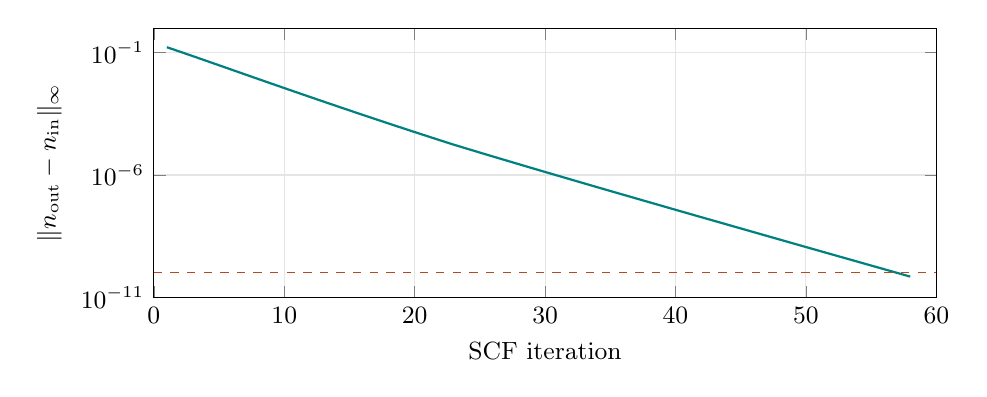
\begin{tikzpicture}
\begin{semilogyaxis}[width=.95\linewidth,height=5.0cm,xlabel={SCF iteration},ylabel={$\|n_{\rm out}-n_{\rm in}\|_\infty$},xmin=0,xmax=60,ymin=1e-11,ymax=1,grid=major,grid style={gray!20},tick label style={font=\small},label style={font=\small}]
\addplot[thick,teal] coordinates {(1,0.16685357) (2,0.11017785) (3,0.072112269) (4,0.047019712) (5,0.030624105) (6,0.019923967) (7,0.012958763) (8,0.0084303705) (9,0.0054981664) (10,0.0035910651) (11,0.0023480775) (12,0.0015372425) (13,0.0010102587) (14,0.0006652255) (15,0.0004387516) (16,0.00029017105) (17,0.00019263823) (18,0.00012813039) (19,8.5387523e-05) (20,5.7173267e-05) (21,3.8367463e-05) (22,2.5798857e-05) (23,1.7423469e-05) (24,1.2012092e-05) (25,8.2882789e-06) (26,5.7364729e-06) (27,3.9819976e-06) (28,2.7657564e-06) (29,1.9220872e-06) (30,1.3384203e-06) (31,9.3478116e-07) (32,6.5309911e-07) (33,4.5645229e-07) (34,3.1912036e-07) (35,2.2352223e-07) (36,1.568674e-07) (37,1.101078e-07) (38,7.7299626e-08) (39,5.4276378e-08) (40,3.8116989e-08) (41,2.6786363e-08) (42,1.8863654e-08) (43,1.3285215e-08) (44,9.3571819e-09) (45,6.5910903e-09) (46,4.6430954e-09) (47,3.2711245e-09) (48,2.3047746e-09) (49,1.6240594e-09) (50,1.1451311e-09) (51,8.0842688e-10) (52,5.7075056e-10) (53,4.0296944e-10) (54,2.8452596e-10) (55,2.0090662e-10) (56,1.4187207e-10) (57,1.0019086e-10) (58,7.0759065e-11)};
\addplot[dashed,warm] coordinates {(0,1e-10) (60,1e-10)};
\end{semilogyaxis}
\end{tikzpicture}
\column{.33\textwidth}
\small
\begin{itemize}
\item $N=4$, $M=8$, $\alpha=0.30$.
\item 58 iterations; final maximum density residual:
$7.08\times10^{-11}$.
\item Also require $|\Delta E|<10^{-12}$ in oscillator energy units.
\item A broadened initial density converges in 63 iterations to the same energy.
\end{itemize}
This is a check of this calculation, not a convergence guarantee for all systems.
\end{columns}
\end{frame}

\begin{frame}{Recomputed energies and checks for the eight-function example}
\begin{center}\small
\begin{tabular}{@{}rrrrr@{}}\toprule
$N$ & $\avg{\hat h_0}$ & $E_H$ & $E_x^{\rm LDA}$ & $E$\\\midrule
1 & 0.50063452 & 0.60855573 & $-0.56165318$ & 0.54753706\\
2 & 2.02320483 & 1.97451757 & $-1.27748570$ & 2.72023670\\
4 & 8.13378445 & 6.42090538 & $-2.86865934$ & 11.68603049\\\bottomrule
\end{tabular}
\end{center}
For $N=4$:
\[
 |\textstyle\int n-4|<10^{-14},\quad
 \|C_{\occ}^\dagger C_{\occ}-I\|<5\times10^{-16},\quad
 |E_{\rm direct}-E_{\rm eig}|=1.09\times10^{-10}.
\]
A density-space finite-difference check of $\delta(E_H+E_x)/\delta n$
agrees with $v_H+v_x$ to $6.9\times10^{-11}$ for the tested direction.
\warnbox{These are energies of the stated approximate functional in a finite
basis. They are not newly claimed exact interacting energies or independent
measurements of functional accuracy.}
\end{frame}

\begin{frame}{Tiny SCF residual does not imply a converged representation}
For $N=4$, the same exchange-only functional gives
\begin{center}\small
\begin{tabular}{@{}lrr@{}}\toprule
Change & Energy & Difference from baseline\\\midrule
$M=8$, 401 nodes, $[-8,8]$ & 11.6860304873 & ---\\
$M=8$, 801 nodes, $[-8,8]$ & 11.6860304873 & $2.5\times10^{-12}$\\
$M=8$, 501 nodes, $[-10,10]$ & 11.6860304873 & $1.8\times10^{-13}$\\
$M=12$, 501 nodes, $[-10,10]$ & 11.6853429697 & $-6.88\times10^{-4}$\\
$M=16$, 501 nodes, $[-10,10]$ & 11.6852955478 & $-7.35\times10^{-4}$\\\bottomrule
\end{tabular}
\end{center}
Doubling the exchange table from 601 to 1201 nodes changes the $M=8$ energy
by $2.2\times10^{-11}$.
\dftbox{Here grid and exchange-table errors are small compared with basis
truncation. A still larger basis would be needed to establish a complete-basis
limit; none of these checks eliminates the functional approximation.}
\end{frame}

\begin{frame}{One particle exposes self-interaction without a many-body ambiguity}
For one particle, the physical two-body operator vanishes. In this trap,
the exact ground-state energy is $E_0=1/2$.
Exact exchange cancels Hartree for its one-particle determinant:
\[
 E_x=-E_H,\qquad E_c=0.
\]
The recomputed local-exchange result instead gives
\[
 E_H+E_x^{\rm LDA}=0.04690255,\qquad
 \avg{\hat h_0}-\frac12=0.00063452,
\]
\[
 \boxed{E^{\rm LDA}-\frac12=0.04753706.}
\]
\begin{itemize}
\item The first number is the self-interaction residue on the computed density.
\item The second is orbital relaxation in $h_0$.
\item For several particles, comparing local and determinant exchange on fixed
orbitals does not cleanly separate locality from self-interaction.
\end{itemize}
\end{frame}

\section{Interpretation and checks}
\begin{frame}{What do Kohn--Sham orbitals and eigenvalues mean?}
The auxiliary system targets the ground-state density; its determinant need
not be the interacting ground-state wave function.
\begin{itemize}
\item KS eigenvalue differences are not generally neutral many-body excitation energies.
\item For an isolated bound atom/molecule, the exact local functional with
the proper potential zero gives $\epsilon_H=-I$ (approach integer $N$ from below).
\item The fundamental charge gap is
\[
 E_g=E(N+1)+E(N-1)-2E(N)=\epsilon_L-\epsilon_H+\Delta_{\xc}.
\]
\item $\Delta_{\xc}$ is the derivative discontinuity. Ordinary smooth LDA/GGA
also have potential errors; not every gap error is solely the missing jump.
\end{itemize}
The isolated-system ionization statement is not a literal interpretation of
the confining oscillator spectrum. Generalized-KS/hybrid spectra require
their own analysis.
\end{frame}

\begin{frame}{A reliable practical calculation separates four tasks}
\begin{enumerate}
\item \textbf{Model:} specify particles, interaction, external potential,
spin, dimensionality, boundaries, and any ionic energy.
\item \textbf{Functional:} state the approximation; derive potentials from
that same energy. Check one-particle and uniform-reference limits.
\item \textbf{Numerics:} converge orbitals, the density fixed point, and the
representation independently. Compare direct and eigenvalue-corrected energies.
\item \textbf{Physics:} examine competing spin/symmetry states and benchmark
observables against reliable references where possible.
\end{enumerate}
\warnbox{An approximate functional is variational with respect to itself,
but generally supplies no rigorous upper bound to the exact interacting
energy. A small residual is not an error bar for that functional.}
\end{frame}

\begin{frame}[fragile]{Summary and the runnable companion}
\begin{itemize}
\item \textbf{HK I:} equal ground-state densities cannot belong to inequivalent
scalar potentials under the stated assumptions.
\item \textbf{HK II:} constrained search proves $E_0=\min_n[F[n]+\int vn]$.
\item \textbf{KS:} define $E_{\xc}=F-T_s-E_H$, vary orthonormal orbitals, and
obtain $v_s=v_{\ext}+v_H+v_{\xc}$.
\item \textbf{Implementation:} build, solve, occupy, compare, mix, and verify;
the total energy is not the raw eigenvalue sum.
\end{itemize}
\begin{lstlisting}
python3 kohn_sham_1d_example.py --output-dir ks_example_results
\end{lstlisting}
\small The companion requires NumPy, SciPy, and Matplotlib. It reproduces
the 1D tables, plots, functional-derivative check, and grid/basis tests in
these slides. This LaTeX source embeds its plotted data and needs no external
figures or original course folders to compile.
\end{frame}

\section{References}
\begin{frame}{References: the foundations and mathematical qualifications}
\small
\begin{thebibliography}{9}
\bibitem{HK} P. Hohenberg and W. Kohn, \emph{Inhomogeneous Electron Gas},
Phys. Rev. \textbf{136}, B864 (1964).
\href{https://doi.org/10.1103/PhysRev.136.B864}{doi:10.1103/PhysRev.136.B864}.
\bibitem{KS} W. Kohn and L. J. Sham, \emph{Self-Consistent Equations Including
Exchange and Correlation Effects}, Phys. Rev. \textbf{140}, A1133 (1965).
\href{https://doi.org/10.1103/PhysRev.140.A1133}{doi:10.1103/PhysRev.140.A1133}.
\bibitem{Levy} M. Levy, \emph{Universal variational functionals of electron
densities, first-order density matrices, and natural spin-orbitals and solution
of the v-representability problem}, PNAS \textbf{76}, 6062 (1979).
\href{https://doi.org/10.1073/pnas.76.12.6062}{doi:10.1073/pnas.76.12.6062}.
\bibitem{Lieb} E. H. Lieb, \emph{Density functionals for Coulomb systems},
Int. J. Quantum Chem. \textbf{24}, 243 (1983).
\href{https://doi.org/10.1002/qua.560240302}{doi:10.1002/qua.560240302}.
\bibitem{Penz} M. Penz et al., \emph{The Structure of the Density-Potential
Mapping. Part I: Standard Density-Functional Theory}, ACS Phys. Chem. Au
\textbf{3}, 334 (2023).
\href{https://doi.org/10.1021/acsphyschemau.2c00069}{doi:10.1021/acsphyschemau.2c00069}.
\end{thebibliography}
\end{frame}

\begin{frame}{References: approximations, eigenvalues, and course connection}
\small
\begin{thebibliography}{9}
\bibitem{PBE} J. P. Perdew, K. Burke, and M. Ernzerhof,
\emph{Generalized Gradient Approximation Made Simple}, Phys. Rev. Lett.
\textbf{77}, 3865 (1996).
\href{https://doi.org/10.1103/PhysRevLett.77.3865}{doi:10.1103/PhysRevLett.77.3865}.
\bibitem{PPLB} J. P. Perdew, R. G. Parr, M. Levy, and J. L. Balduz,
\emph{Density-Functional Theory for Fractional Particle Number: Derivative
Discontinuities of the Energy}, Phys. Rev. Lett. \textbf{49}, 1691 (1982).
\href{https://doi.org/10.1103/PhysRevLett.49.1691}{doi:10.1103/PhysRevLett.49.1691}.
\bibitem{SS} L. J. Sham and M. Schl\"uter, \emph{Density-Functional Theory of
the Energy Gap}, Phys. Rev. Lett. \textbf{51}, 1888 (1983).
\href{https://doi.org/10.1103/PhysRevLett.51.1888}{doi:10.1103/PhysRevLett.51.1888}.
\bibitem{course} C. Glittum and M. Hjorth-Jensen, supplied
\texttt{week42.tex} and \texttt{week43.tex}; M. Hjorth-Jensen,
\texttt{BookPrograms/chapter08/dft.py}. These supply the visual template,
course progression, and 1D teaching Hamiltonian.
\bibitem{rdm} \emph{From the many-body wave function to densities}, supplied
one- and two-body RDM supplement. The ordered-pair convention and the
distinction between the local density and the RDMs are retained here.
\end{thebibliography}
\end{frame}

\end{document}
